Po analýze tvorby dokumentů a nástrojů na vytváření dokumentů připravíme návrh aplikace, která bude řešit správu, vytváření a verzování
modulárních dokumentů. Tato kapitola je rozdělena do jednotlivých sekcích, ve kterých budeme podrobně popisovat návrh dané sekce v naší aplikaci.
V~rámci návrhu nesmíme opomenout možnosti budoucího rozšíření.

\section{Uživatelská sekce}

Tato sekce je zde hlavně pro potřeby vytváření neveřejných dokumentů, které nesmí být přístupné veřejnosti. Dále je také potřeba vytvořit možnost
správy systému, která bude jednoduchá na použítí a nebude nutné například zasahovat přímo do databáze naší aplikace. Pro tuto funkcionalitu bude ovšem
nutné vytvořit speciální roli, která bude tohoto administrátora jasně identifikovat. Role ale nebude pouze administrátorská, všichni uživatelé budou mít
možnost být nositeli až několika rolí zároveň. Tato vlastnost je zde kvůli jednodušší obsluze přiřazování oprávnění k dokumentům a repozitářům, které si rozebereme
dále v textu. Aby hlavní administrátor aplikace nemusel tyto požadavky na přidělení rolí řešit sám, bude zde ještě další pevně definovaná role a to role
správce přístupu, který bude mít možnost, stejně jako administrátor, hromadně přidělovat či odebírat role. Ovšem pouze administrátor může přiřadit roli správce přístupu.

Nyní si probereme vlastnosti uživatele, budeme potřebovat uživatele jednoznačně identifikovat, je tedy potřeba od uživatele získat nějaký údaj, který bude unikátní
jako například uživatelské jméno. Dále si od uživatele vyžádáme email, který může být posléze použit k doručení zpráv a upozornění z~aplikace. Tímto se ovšem
dostáváme k nutnosti myslet na ochranu osobních údajů, která prošla v posledních letech změnou v důsledky nabytí účinosti evropského nařízení \gls{gdpr}.

V~tomto UC diagramu \ref{fig:userUCDiagram} naleznete rozpis všech UC, které se týkají uživatelské sekce. Zároveň k tomu je zde také stavový diagram \ref{fig:userFlow},
který nám ukazuje jednotlivé stavy uživatele, vzhledem k systému a které akce mají vliv na jeho stav.

\begin{figure}[H]
    \centering
    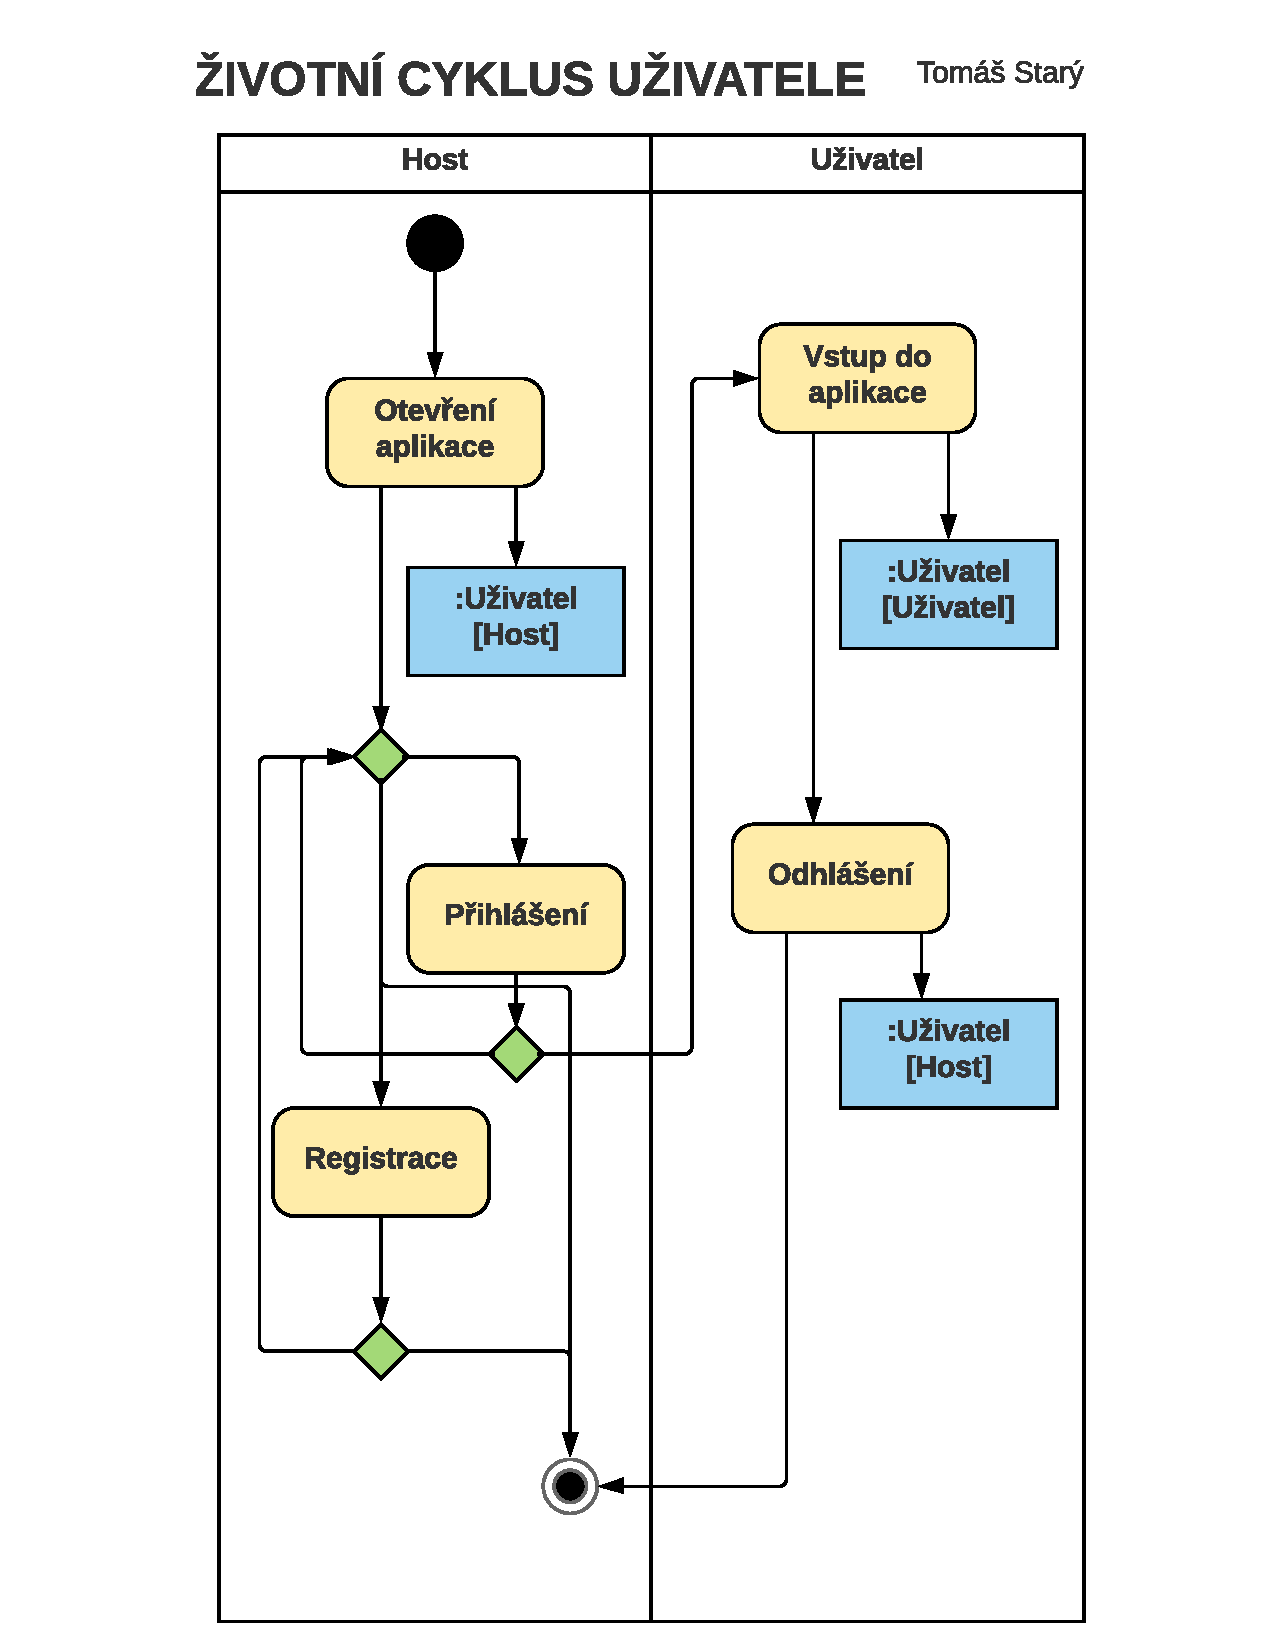
\includegraphics[width=\textwidth]{lifecycle.pdf}
    \caption{Diagram přihlášení a registrace uživatele}
    \label{fig:userFlow}
\end{figure}

\begin{figure}[h]
    \centering
    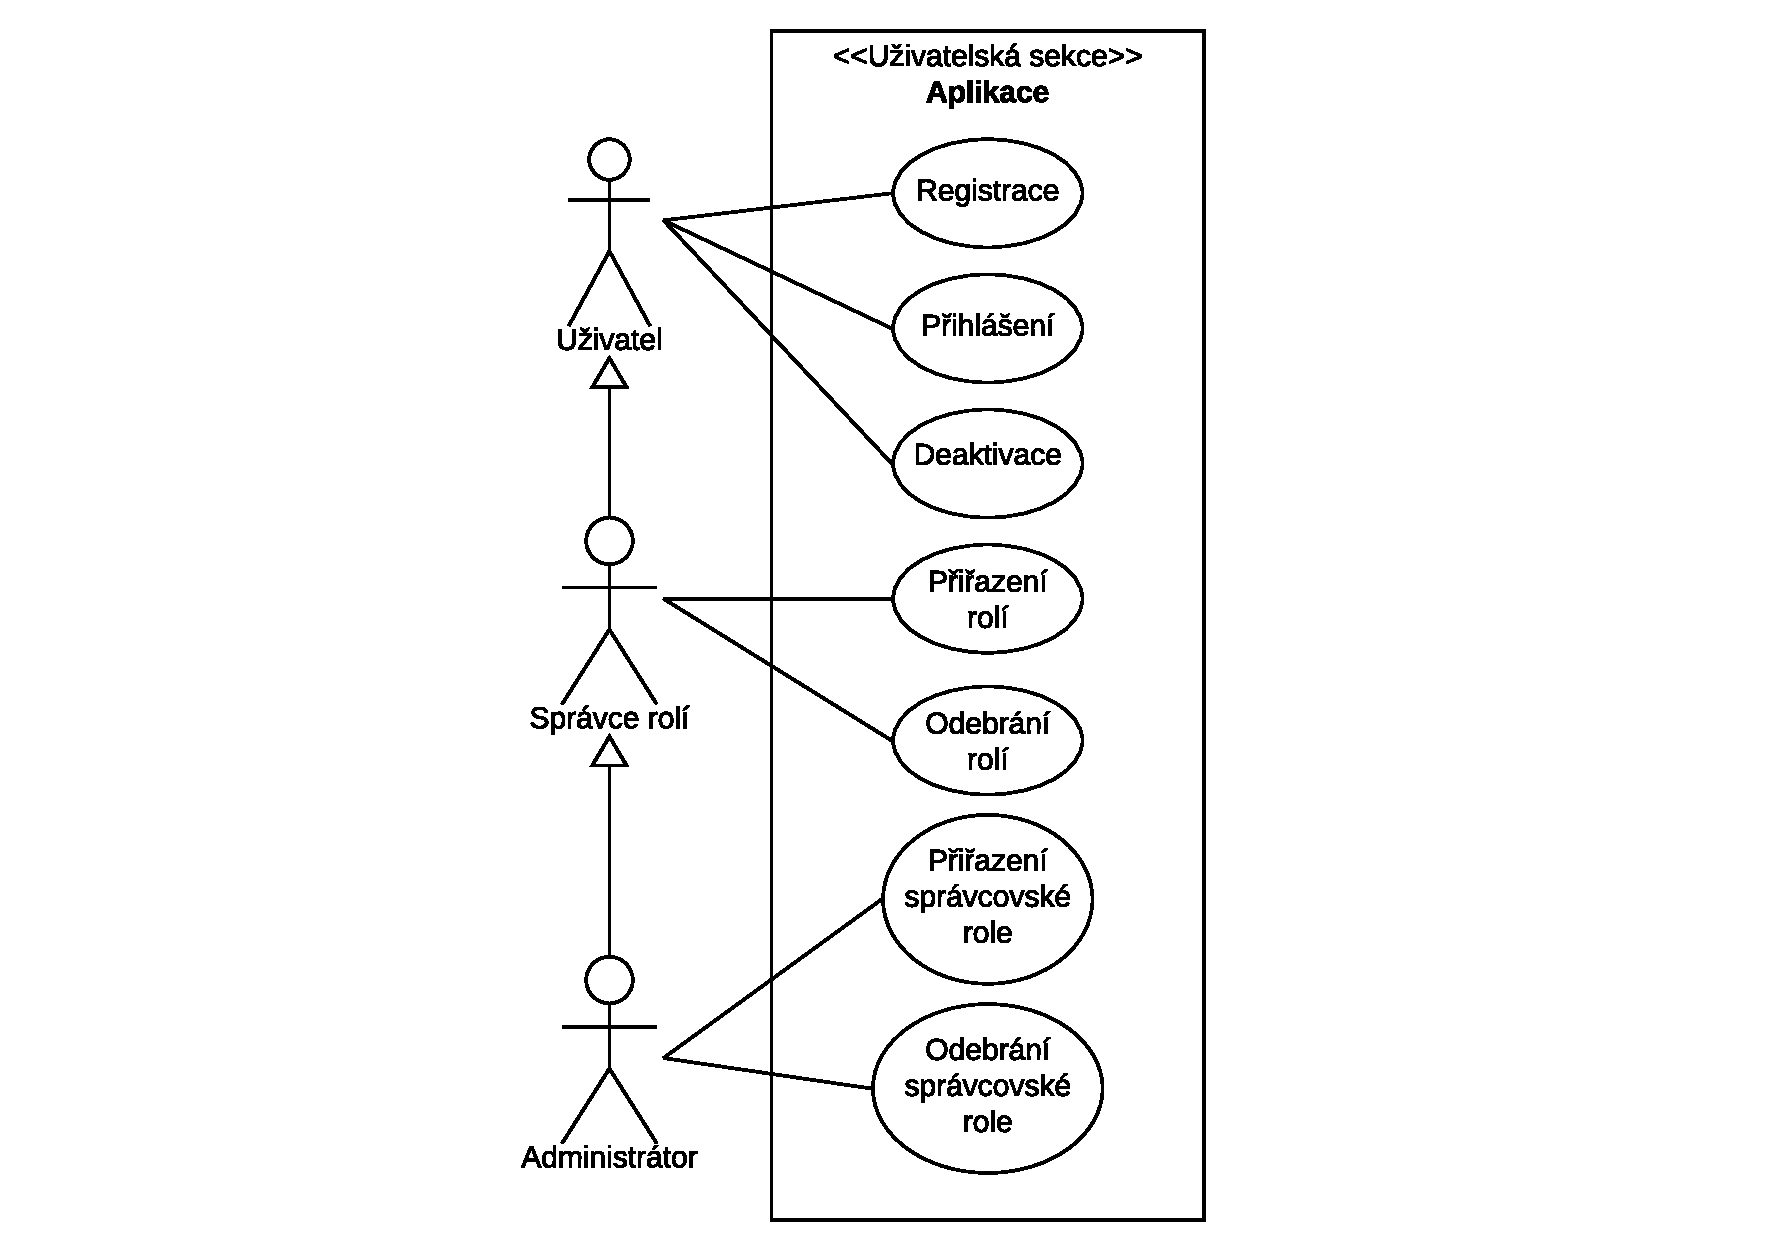
\includegraphics[width=\textwidth]{userUCDiagram.pdf}
    \caption{Diagram UC pro uživatelskou sekci}
    \label{fig:userUCDiagram}
\end{figure}

\subsection{\gls{gdpr}}

Naše aplikace bude pracovat s osobními údaji, je nutné toto brát na~vědomí. Proto se nyní podívejme na to, co musí naše aplikace splňovat, aby dodržela všechny
zákony o ochraně osobních údají a směrnice Evropské unie, \gls{gdpr}. První co je nutné brát na vědomí je účel, za kterým údaje chceme údaje sbírat a uchovávat a jestli je náš
účel oprávněný. V tomto případě o uživateli získáme osobní údaj v podobě emailu, který stačí k identifikaci určité osoby. V~našem případě je email identifikátor uživatele
a budeme jej při registraci žádat o~\mbox{souhlas} se zpracováním osobních údajů. Dále musíme myslet na\linebreak možnost smazání či anonymizace údajů uživatele. Toho docílíme ručními
zá\-sahy do databáze, kde využijeme možnosti změnit email na jeho hash. \cite{gdpr}

\section{Repozitáře}

Než začneme popisovat samotné generování dokumentů, je potřeba si \mbox{definovat} repozitáře našich modulů. Jednotlivé repozitáře nám budou sloužit jako složky,
které budou obsahovat moduly, ze kterých se pak budou skládat výsledné dokumenty. V rámci repozitářů je potřeba hlavně zajistit správně fungování oprávnění.
Pokud si uživatel založí nový repozitář, má vůči němu všechny práva, ostatní uživatelé se namejí o tomto repozitáři v tomto stavu nemají jak dozvědět, je pro ně
skrytý. Pokud se ovšem zakladatel rozhodne svůj obsah repozitáře sdílet, má možnost sdílet repozitář s ostatními uživateli.
Dále má také možnost definovat, jestli je repozitář pro jednotlivé uživatele pouze pro čtení, či použití modulu v dokumentu,
nebo jestli má možnost moduly i upravovat.

V neposlední řadě musíme myslet na verzování našich jednotlivých modulů, zde se nabízejí 2 možnosti jak tomuto přistoupit. Buď by bylo možné integrovat
řešení založené na nějaké \gls{vcs}, tj. systém, který zařizuje verzování souborů,
nebo je možné implementovat verzování pomocí databáze. V této práci budeme volit verzování pomocí databáze a to hlavně z časových důvodů, neboť
pro použití \gls{vcs} by bylo nutné udělat kompletní obal na nějaký již existující verzovací systém. Na digramu \ref{fig:moduleDia} je vidět, jak by měly
vypadat vztahy mezi jednotlivými moduly.

Pro jednodušší představu toho jaké nám z návrhu vyplynuly příklady užití je vytvořen diagram UC pro repozitáře \ref{fig:repositoryUC}. V tomto diagramu je dbáno i na rozdělení
uživatelů podle úrovně jejich oprávnění ve vztahu k repozitáři.

\begin{figure}[H]
    \centering
    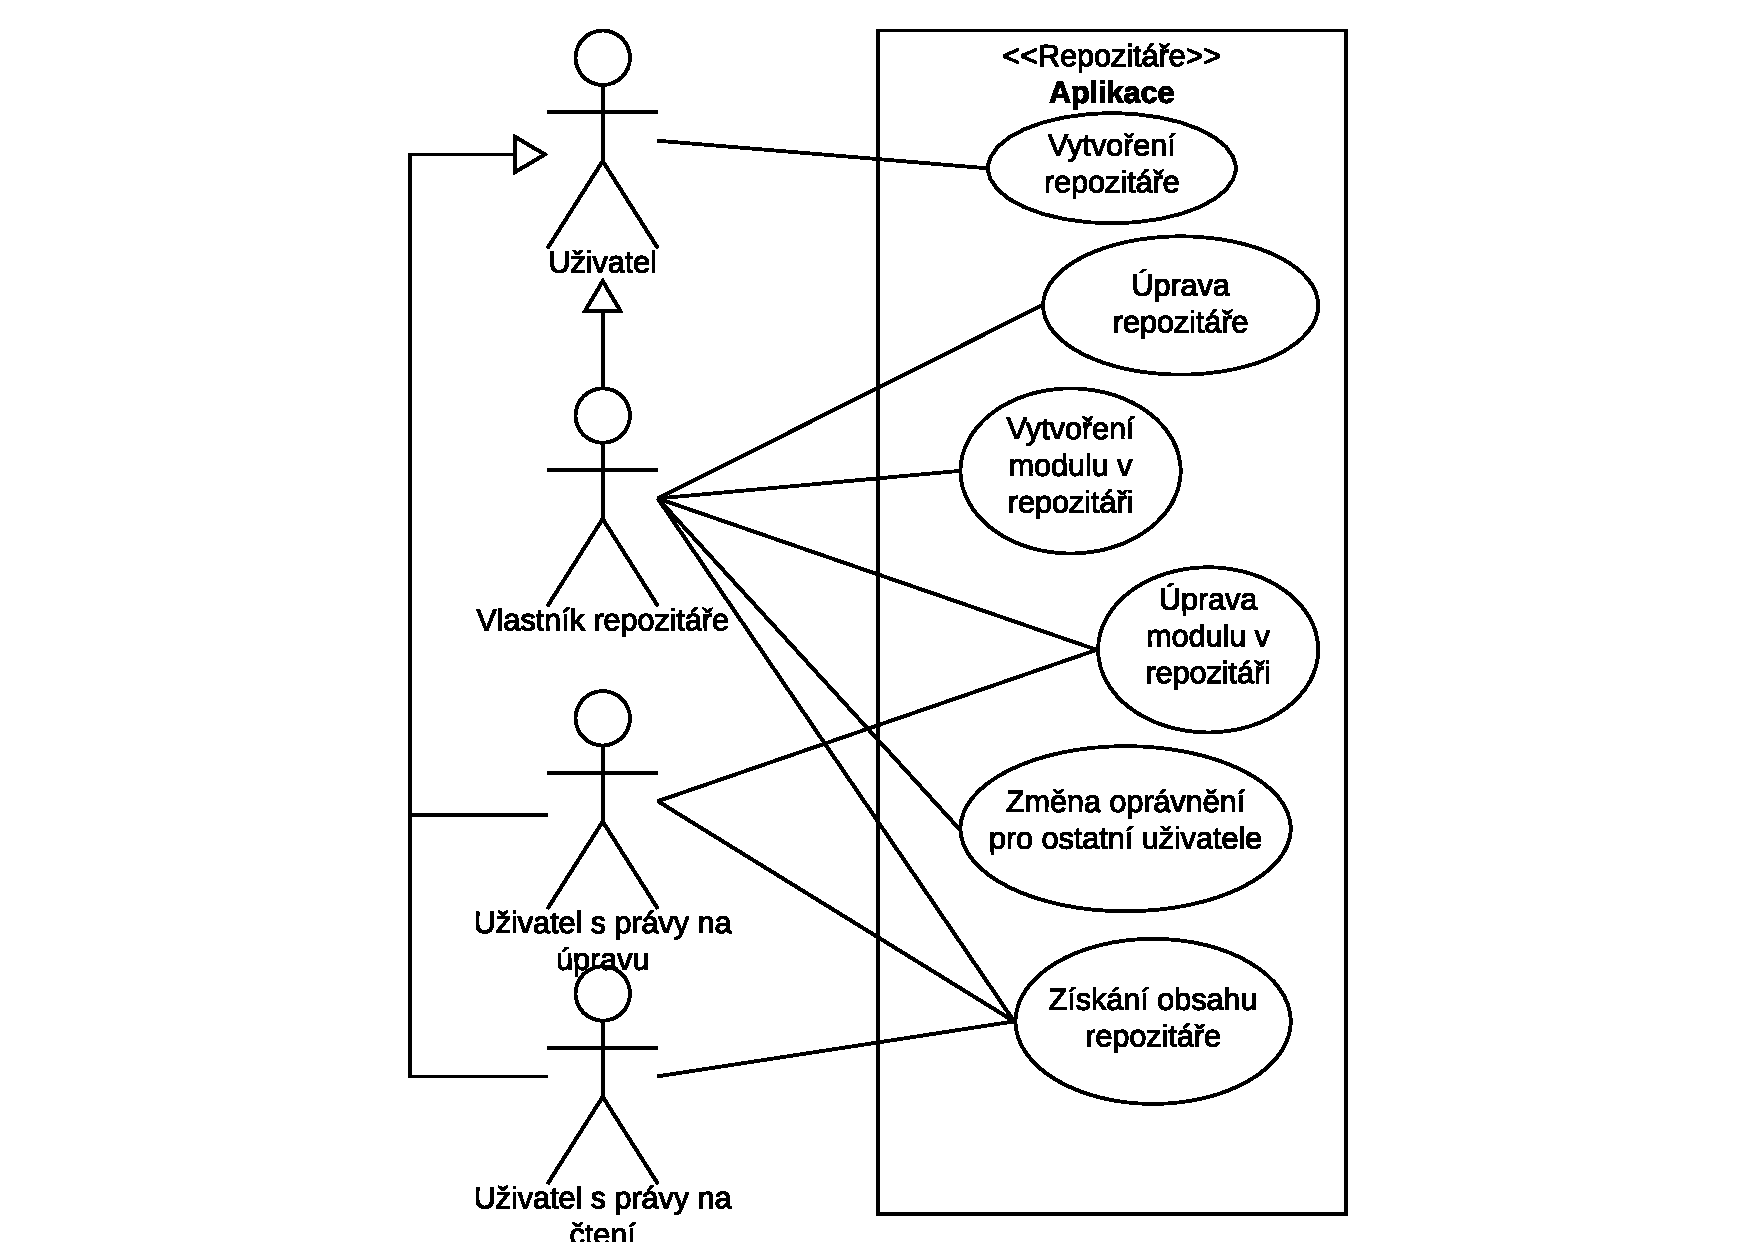
\includegraphics[width=\textwidth]{repositoryUCDia.pdf}
    \caption{Diagram UC pro repozitáře}
    \label{fig:repositoryUC}
\end{figure}

\section{Dokumenty}

Jelikož už máme definované chování pro jednotlivé repozitáře a jejich moduly, můžeme se pustit do návrhu dokumentů, které se budou skládat z modulů. Každý
dokument je tedy soubor modulů, který je možné převést do tisknutelné podoby. Co ale nesmíme opomenout je, že stejně jako moduly bude možné dokumenty také
verzovat, zde to bude provedeno pomocí revizí. Každá revize bude nést informace o tom, kdo danou revizi vytvořil a také ponese všechny informace o verzích
modulu, které jsou na danou revizi použity.

Podobně jako u repozitářů i u dokumentů budeme řešit oprávnění a to stejným způsobem, tudíž každý dokument má svého zakladatele nebo také vlastníka,
vlastník má možnost rozhodovat o tom, kdo bude moci dokument upravovat (vytvářet nové revize, měnit obsah dokumentu), a kdo bude mít možnost si pouze dokument
přečíst.

Pro lepší představu o jednotlivých případech užití je zde přiložen UC diagram pro dokumenty \ref{fig:documentUC}.

\begin{figure}[H]
    \centering
    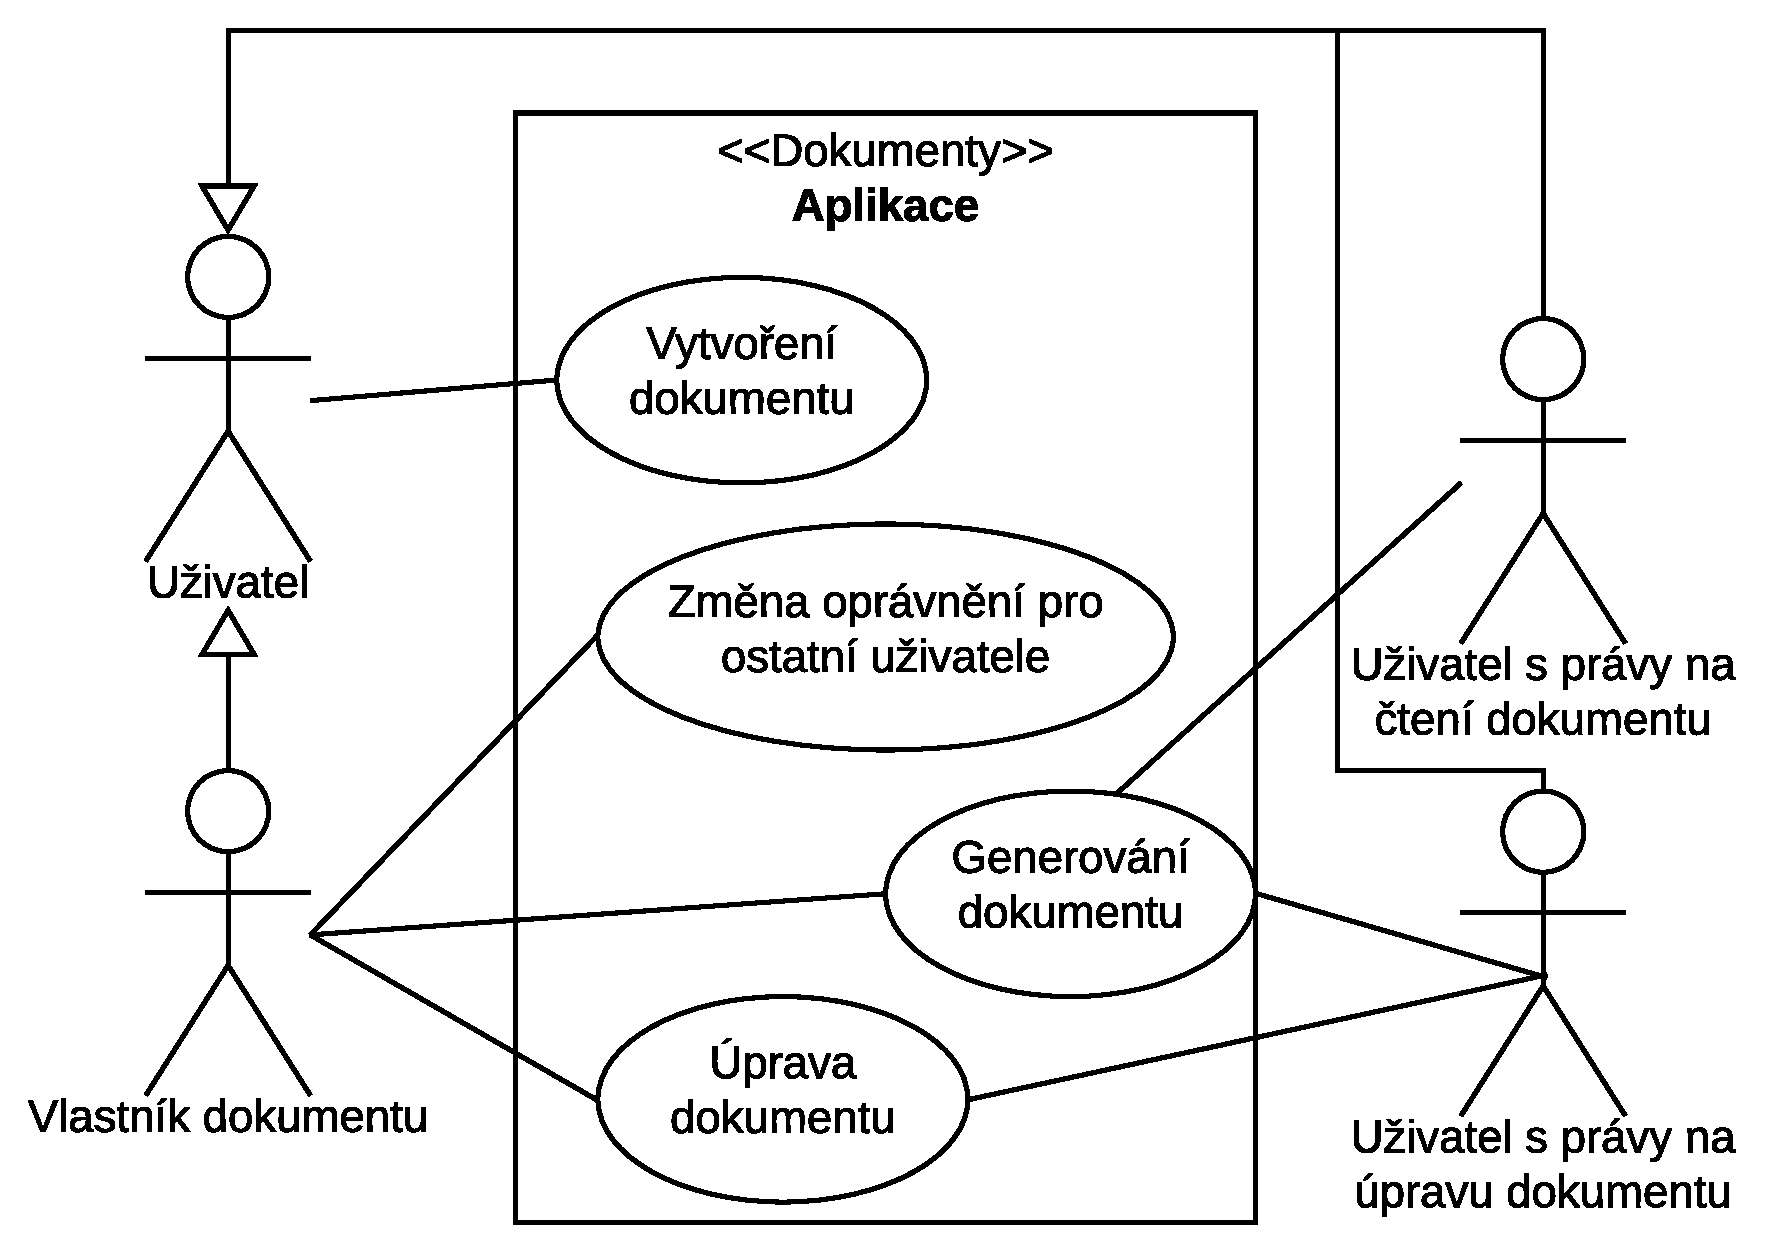
\includegraphics[width=\textwidth]{documentUCDia.pdf}
    \caption{Diagram UC pro dokumenty}
    \label{fig:documentUC}
\end{figure}

\section{Návrh architektury aplikace}

Jak bylo již řečeno v kapitole o cílech práce, aplikace by měla být rozdělena na 2 části backend a frontend. Nyní si pojdmě navrhnout architekturu, která bude
vyhovovat tomuto cíly. Pro backend je důležité, aby měl přístup k databázi, ve~které budou uložena všechna data, jediná možnost jak komunikovat s backendem bude
skrze webové rozhraní. Propojeni s backendem nám bude zajišťovat frontendová část, ta bude umět komunikovat a zobrazovat data v~grafické podobě, nadále nám také
poslouží k udržení identity po přihlášení. Na tomoto diagramu \ref{fig:softCompDia} je znázorněno rozložení jednotlivých komponent dle návrhu.

\begin{figure}[H]
    \centering
    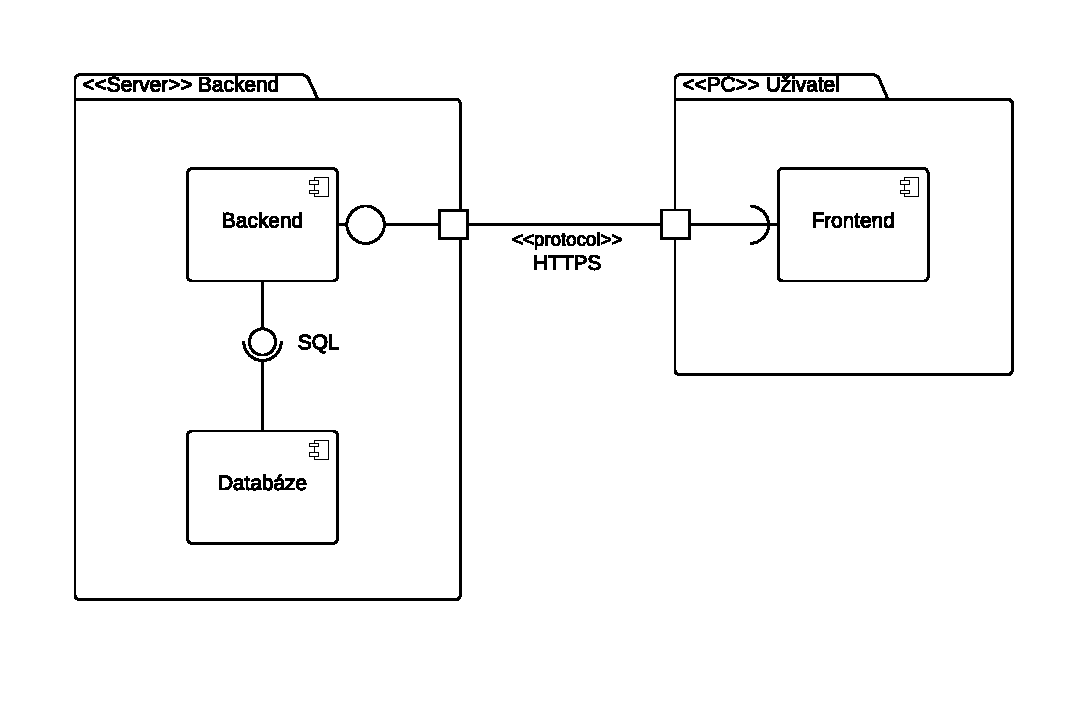
\includegraphics[width=\textwidth]{soft_comp_dia.pdf}
    \caption{Diagram komponent}
    \label{fig:softCompDia}
\end{figure}

\section{Možnosti rozšíření}

Protože každý systém se postupně rozvíjí a rozšiřuje, musíme na tuto skuteč\-nost myslet již při návrhu, snažíme se tedy, aby jednotlivé části systému byly od sebe
oddělené a mohly fungovat i bez ostatních částí. Například propojení mezi moduly a uživateli je pouze na základě jedné vazební tabulky, která slouží k~dekompozici vztahu
M:N. U modulů je také podstatné, aby bylo možné jim v dalším vývoji přidat další atributy jako například typ modulu. Toho docílíme tím, že moduly budou samostatnou tabulkou v databázi
a bude ji tedy možné rožšířit o další atributy, při této úpravě ovšem neohrozíme již původní data a nebude pro nás problém takovou změnu implementovat. Podobně je tomu i u~dokumentů a uživatelů.
Modely se snažíme dělat co nejmenší s jednoduchou možností rozšíření viz \ref{fig:moduleDia}.

\begin{figure}[h]
    \centering
    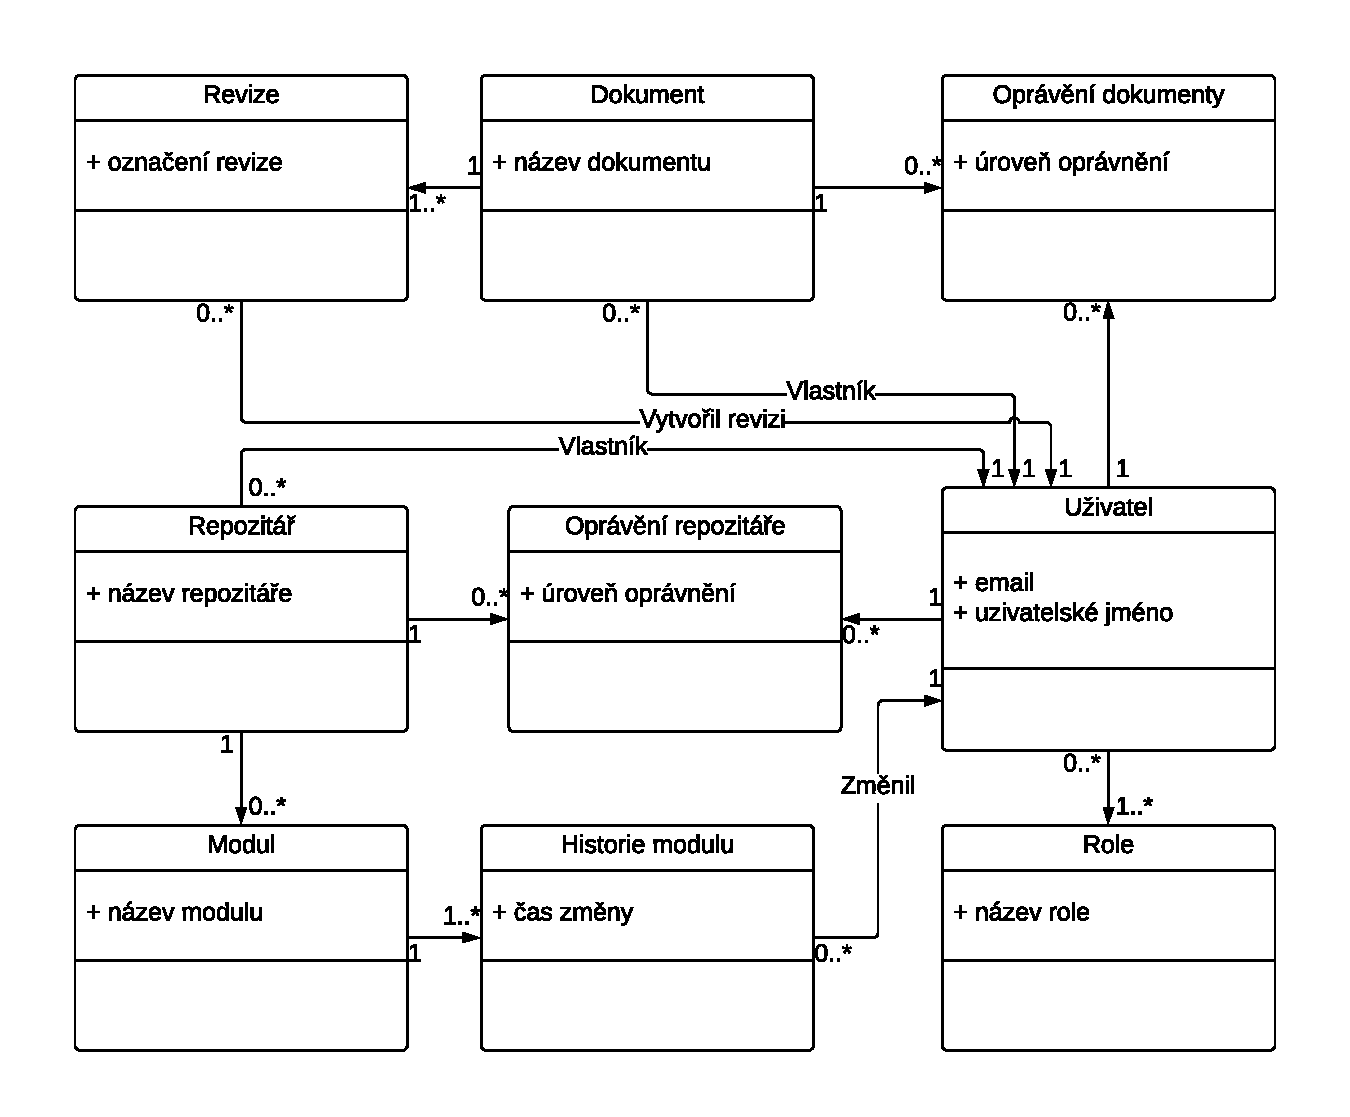
\includegraphics[width=\textwidth]{module_diagram.pdf}
    \caption{Návrh rozložení modelů}
    \label{fig:moduleDia}
\end{figure}